\section{表面反射}\label{sec:表面反射}

当光入射到表面时,表面会散射该光,将其一部分反射回环境中。
有两个需要描述的效应以对反射建模:反射光的光谱分布和其方向分布。
例如,柠檬皮大都吸收了蓝波长的光而反射了大部分红和绿波长的光
(回想\reffig{5.1}中柠檬皮的反射SPD)。
因此,当用白光照射它时,其颜色是黄色。
无论从哪个方向观察,皮的颜色都相当一致,
但有的方向会有\keyindex{高光}{highlight}{}——会看见与其说黄色不如说白色的更亮区域
\sidenote{译者注:有高光区的柠檬照片。}。
\begin{marginfigure}
    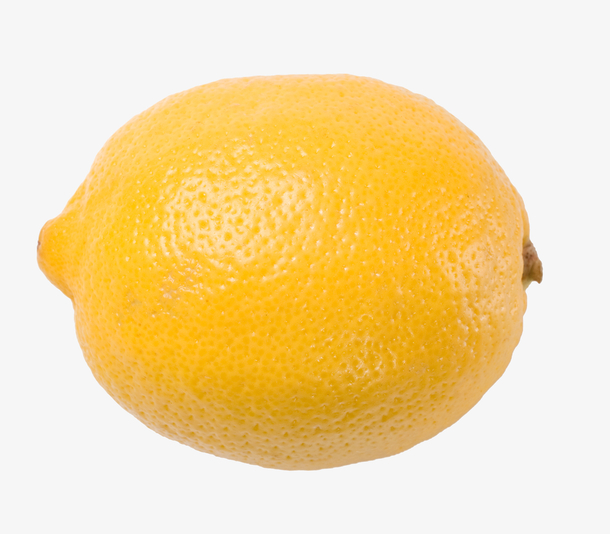
\includegraphics[width=\linewidth]{chap05/lemon.jpg}
\end{marginfigure}
相反,镜子一点反射的光几乎完全取决于观察方向。
在镜子的固定点上,当观察角度变化时,镜子反射的物体也随之变化。

来自\keyindex{半透明}{translucent}{}表面的反射更复杂;
从皮和叶子到蜡和液体的各种材料都
表现出\keyindex{次表面光传输}{subsurface light transport}{light transport光传输},
即进入表面一点的光在有一定距离的地方退出。
(例如考虑在一个人的嘴巴里开手电筒会让他的脸颊被照亮,
因为进入脸颊内侧的光穿过了皮肤并从脸上退出。)

有两种抽象来为光的反射描述这些机制:
\refsub{BRDF}和\refsub{BSSRDF}分别介绍的BRDF和BSSRDF。
BRDF描述一点的表面反射而忽略次表面光传输效应;
对于不受该传输机制明显影响的材料,
这一简化会减少报错并让渲染算法的实现高效得多。
BSSRDF推广了BRDF并描述来自半透明材料光反射的更一般设置。

\subsection{BRDF}\label{sub:BRDF}
\keyindex{双向反射分布函数}{bidirectional reflectance distribution function}{}(BRDF)
为描述来自表面的反射给出了形式。考虑\reffig{5.18}中的设置:
我们想知道,作为沿方向${\bm\omega}_{\mathrm{i}}$
入射辐亮度$L_{\mathrm{i}}({\bm p},{\bm\omega}_{\mathrm{i}})$的结果,
在朝向观察者的方向${\bm\omega}_{\mathrm{o}}$中
有多少辐射亮度$L_{\mathrm{o}}({\bm p},{\bm\omega}_{\mathrm{o}})$离开表面。
\begin{figure}[htbp]
    \centering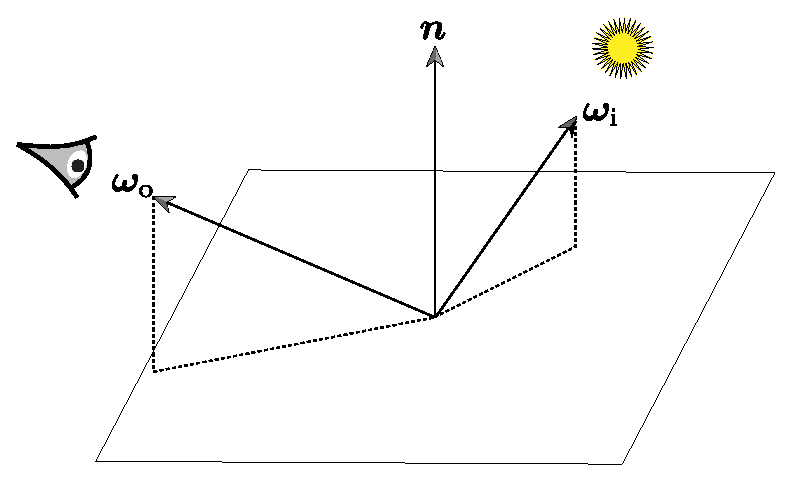
\includegraphics[width=0.5\linewidth]{chap05/BRDF.eps}
    \caption{BRDF。双向反射分布函数是在一对方向${\bm\omega}_{\mathrm{i}}$
        和${\bm\omega}_{\mathrm{o}}$上描述有多少沿${\bm\omega}_{\mathrm{i}}$
        入射的光从表面朝方向${\bm\omega}_{\mathrm{o}}$散射的4D函数。}
    \label{fig:5.18}
\end{figure}

如果方向${\bm\omega}_{\mathrm{i}}$视作方向的微分锥,则$\bm p$处的微分辐照度是
\begin{align}\label{eq:5.7}
    \mathrm{d}E({\bm p},{\bm\omega}_{\mathrm{i}})=L_{\mathrm{i}}({\bm p},{\bm\omega}_{\mathrm{i}})\cos\theta_{\mathrm{i}}\mathrm{d}{\bm\omega}_{\mathrm{i}}\, .
\end{align}

要被反射到方向${\bm\omega}_{\mathrm{o}}$的辐射亮度微分量取决于该辐射照度。
因为几何光学的线性假设,反射的微分辐射亮度正比于辐射照度
\begin{align*}
    \mathrm{d}L_{\mathrm{o}}({\bm p},{\bm\omega}_{\mathrm{o}})\propto\mathrm{d}E({\bm p},{\bm\omega}_{\mathrm{i}})\, .
\end{align*}

比例常数为这对特定方向${\bm\omega}_{\mathrm{i}}$和${\bm\omega}_{\mathrm{o}}$定义了曲面的BRDF:
\begin{align}\label{eq:5.8}
    f_{\mathrm{r}}({\bm p},{\bm \omega}_\mathrm{o},{\bm \omega}_\mathrm{i})=\frac{\mathrm{d}L_{\mathrm{o}}({\bm p},{\bm\omega}_{\mathrm{o}})}{\mathrm{d}E({\bm p},{\bm\omega}_{\mathrm{i}})}=\frac{\mathrm{d}L_{\mathrm{o}}({\bm p},{\bm\omega}_{\mathrm{o}})}{L_{\mathrm{i}}({\bm p},{\bm\omega}_{\mathrm{i}})\cos\theta_{\mathrm{i}}\mathrm{d}{\bm\omega}_{\mathrm{i}}}\, .
\end{align}

基于物理的BRDF有两个重要性质:
\begin{enumerate}
    \item \keyindex{互易性}{reciprocity}{}:对所有方向对${\bm\omega}_{\mathrm{i}}$和${\bm\omega}_{\mathrm{o}}$,
          $f_{\mathrm{r}}({\bm p},{\bm \omega}_\mathrm{i},{\bm \omega}_\mathrm{o})=f_{\mathrm{r}}({\bm p},{\bm \omega}_\mathrm{o},{\bm \omega}_\mathrm{i})$。
    \item {\sffamily 能量守恒}:光反射的总能量少于或等于入射光的能量。
          对于所有方向${\bm\omega}_{\mathrm{o}}$,
          \begin{align*}
              \int\limits_{H^2({\bm n})}f_{\mathrm{r}}({\bm p},{\bm \omega}_\mathrm{o},{\bm \omega}')\cos\theta'\mathrm{d}{\bm\omega}'\le1\, .
          \end{align*}
\end{enumerate}

曲面的\keyindex{双向透射分布函数}{bidirectional transmittance distribution function}{}(BTDF)
描述透射光的分布,可以用和BRDF一样的方法定义。

\subsection{BSSRDF}\label{sub:BSSRDF}